\documentclass[11pt, titlepage]{article}

% Math text
\usepackage[utf8]{inputenc}
\usepackage[a4paper,
            top=2cm,bottom=2cm,
            margin=3.5cm,
            headheight=27pt]{geometry}
\usepackage[spanish, mexico]{babel}
%\usepackage[utopia]{mathdesign}
\usepackage{amsmath,amssymb,array,siunitx}
% HEADER
\usepackage{fancyhdr,framed}
\setlength{\headheight}{44pt}
\pagestyle{fancy}
\usepackage[T1]{fontenc}
\usepackage[utf8]{inputenc}
\usepackage{soulutf8,xcolor}
\usepackage{svg}
\usepackage{graphicx}

% !TeX root = control_rapido.tex
%% DIFFERENTIAL OPERATOR
\makeatletter
\providecommand*{\diff}%
{\@ifnextchar^{\DIfF}{\DIfF^{}}}
\def\DIfF^#1{%
	\mathop{\mathrm{\mathstrut d}}%
	\nolimits^{#1}\gobblespace}
\def\gobblespace{%
	\futurelet\diffarg\opspace}
\def\opspace{%
	\let\DiffSpace\!%
	\ifx\diffarg(%
	\let\DiffSpace\relax
	\else
	\ifx\diffarg[%
	\let\DiffSpace\relax
	\else
	\ifx\diffarg\{%
	\let\DiffSpace\relax
	\fi\fi\fi\DiffSpace}


\newcommand{\dimfont}[1]{\ensuremath{#1}}
\newcommand{\Cme}[1]{\mathbf{#1}}
\newcommand{\Mme}[1]{\mathbf{#1}}
\newcommand{\Ts}{T_s}

\newcommand{\eye}{\Mme{I}}
%transpose
\def\dt{\Delta t}
\def\tp{^{\top}}
% Small
\def\MA{\Mme{A}}
\def\MB{\Mme{B}}
\def\MC{\Mme{C}}
\def\MD{\Mme{D}}
\def\ME{\Mme{E}}
\def\MK{\Mme{K}}
\def\MW{\Mme{W}}
\def\MX{\Mme{X}}
\def\MV{\Mme{V}}
\def\ctrb{\Mme{Y}}
\def\Mzero{\Mme{0}}
\def\obsv{\Mme{\mathcal{O}}}

\newcommand{\ts}[2]{\left. #1\right|_{\tiny #2}}

\def\error{\varepsilon}
\def\Cx{\Cme{x}}
\def\Cf{\Cme{f}}
\def\Cy{\Cme{y}}
\def\Cu{\Cme{u}}
\def\Cn{\Cme{n}}
\def\Cd{\Cme{d}}
\def\Czero{\Cme{0}}
\def\Cv{\Cme{v}}
\def\Cz{\Cme{z}}
\def\Cw{\Cme{w}}
\def\Jcost{\Cme{\mathcal{J}}}
% RK4
\def\Ca{\Cme{a}}
\def\Cb{\Cme{b}}
\def\Cc{\Cme{c}}


\def\noise{{n}}
\def\disturb{{d}}
\newcommand{\di}{\ensuremath{\textrm{d}}}

\newcommand{\Matlab}{{\sc Matlab}}

\newcommand{\spartial}[2]{\frac{\partial {#1}}{\partial {#2}}}
\newcommand{\dpartial}[2]{\frac{\partial^2 #1}{\partial #2 ^2}}

\usepackage{amsthm}
\theoremstyle{definition}
\newtheorem{definition}{Definition}[chapter]
\newtheorem{theorem}{Teorema}[chapter]
\newtheorem{exercise}{Ejercicio}[chapter]

\lhead{ Patricio Whittingslow \\ Agustín Canalis}


%\usepackage{bigfoot} % to allow verbatim in footnote
\usepackage[numbered,framed]{matlab-prettifier}



\let\ph\mlplaceholder % shorter macro
\lstMakeShortInline"
\renewcommand{\lstlistingname}{Código}
\renewcommand{\lstlistlistingname }{Códigos \Matlab}
\lstset{
  style              = Matlab-editor,
  basicstyle         = \mlttfamily,
  escapechar         = ",
  mlshowsectionrules = true,
  numbers = none,
  tabsize=4,
}



\begin{document}
%Caratula
\begin{titlepage}

\centering
{\small Instituto Tecnológico de Buenos Aires \par}


\vspace{8cm}
{\Huge Método de volúmenes finitos para transferencia de calor en sólidos \par}
\vspace{2cm}
{ \large {Patricio Whittingslow   \\
 Agustín Canalis\par}}
\vspace{4cm}
\today

\end{titlepage}
%

\section*{Glosario}


\glossentry{\Cme{X}}{Vector columna X}
\glossentry{\Mme{X}}{Matriz X}
\glossentry{\Cme{T}^{m+1}}{Vector temperaturas evaluado en el instante de tiempo discretizado $m+1$}
\glossentry{\Mme{C} \mldivide  \Cme{A} }{Resolución del sistema de ecuaciones para obtener el vector $\Cme{B}$ donde $\Mme{C}\Cme{B}=\Cme{A}$. Es equivalente a $\Mme{C}^{-1}\cdot \Cme{A} $}
\subsection*{Notas}
Los superíndices con $m$ se refieren a la discretización temporal. Los subíndices $\vol,\north,\south,\east,\west$ se refieren a la discretización espacial. Dicho subíndice $\vol$ se refiere al volumen en cuestión donde se está haciendo el balance de energía; los volúmenes $\north,\south,\east,\west$ se refieren a los vecinos de este último. 

\section{Discretización de la ecuación de calor}
Se comienza con la ecuación de Fourier para un sólido con calor generado.
\begin{equation}\label{eq:fourier}
    \spartial{T}{t} = \frac{ k }{\rho \cp} \nabla^2 T + \qG
\end{equation}

Generalizándola para un volumen arbitrario $\di V$ 
\begin{equation} \label{eq:fourierVolumenes}
     \rho \cp \spartial{T}{t} \di V = k \spartial{T}{x} \di S + \qG \di V
\end{equation}
la cual se puede trabajar con un sistema cartesiano e integrar para llegar a la ecuación de Fourier discretizada para volúmenes finitos

\begin{equation}
        \frac{V\rho \cp}{\Delta t}\left(T_\vol^{m+1}-T_\vol^{m} \right) = \sum_i^{\text{caras}} k\cdot S_i\frac{(T_i-T_\vol)}{\Delta x_i}+\!  \qG V 
\end{equation}

El esquema explicito (ecuación \ref{eq:discretizadaExplicito}) para resolver la ecuación diferencial numéricamente obtiene las temperaturas en el próximo paso de tiempo con las temperaturas inmediatas
\begin{equation} \label{eq:discretizadaExplicito}
    \frac{V\rho \cp}{\Delta t}\left(T_\vol^{m+1}-T_\vol^{m} \right) = \left.\sum_i^{\text{caras}} k\cdot S_i\frac{(T_i-T_\vol)}{\Delta x_i}\right|^{m} +\!\! \left. \qG V \right|^{m}
\end{equation}
tiene la ventaja de ser fácil de programar por su naturaleza intuitiva y de dar resultados precisos. Además, es paralelizable ya que las temperaturas futuras son independientes entre sí. Aún así, tiene la gran desventaja de ser inestable si se discretiza con un número Fourier lo suficientemente alto.

El esquema implícito (ecuación \ref{eq:discretizadaImplicita}) es menos fácil de visualizar, pues las temperaturas del futuro dependen entre sí. Esto también lo hace imposible de paralelizar.
\begin{equation} \label{eq:discretizadaImplicita}
    \frac{V\rho \cp}{\Delta t}\left(T_\vol^{m+1}-T_\vol^{m} \right) = \left.\sum_i^{\text{caras}} k\cdot S_i\frac{(T_i-T_\vol)}{\Delta x_i}\right|^{m+1} +\!\! \left. \qG V \right|^{m+1}
\end{equation}
pero si no se mira la mosca en la sopa, tiene la ventaja de ser estable.

\section{Programación del FVM}
\subsection{Dominio}
Por simplicidad se detallar el método de volúmenes finitos formulado para un problema 2-D. Primero se define el dominio. En la figura se encuentra una placa que tiene $L_x$ de largo, $L_y$ de alto, $e$ de espesor y está dividida en 6 volúmenes cuadrados. El hecho que sean cuadrados simplificará los cálculos más adelante.
\subsection{Condiciones de borde}
El próximo paso es definir el modelo matemático, es decir, condiciones de borde de Dirichlet y de Neumann. Tenemos los dos costados aislados y el borde superior de la placa a una temperatura $T_H$ y el borde inferior a una temperatura $T_C$ como se puede ver en la figura \ref{fig:simpleDomain}. Se tiene entonces condiciones de borde de Neumann sobre la caras de costado (\east{} y \west{}) y condiciones de borde de Dirichlet en la superior e inferior.


\begin{figure}[htb!]
    \centering
    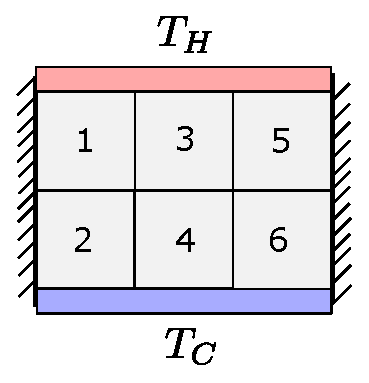
\includegraphics[width=5cm]{fig/simpleDomain.eps}
    \caption{Un dominio simple.}
    \label{fig:simpleDomain}
\end{figure}

\subsection{La matriz \texttt{vecindario}}
Llegado a este punto se puede comenzar la programación. Resulta visualmente cómodo plantear un sistema de orientación con las direcciones cardinales. En 2D se tiene el norte, oeste, este y sur, según sus contrapartes en ingles: N,W,E,S (figura \ref{fig:nsew}). Esto nos va ayudar indexar que volúmenes comparten una frontera en la matriz \texttt{vecindario}, dicho de otra forma, cuales son los \texttt{vecinos} de un volumen \textbf{V}.

\begin{figure}[htb!]
    \centering
     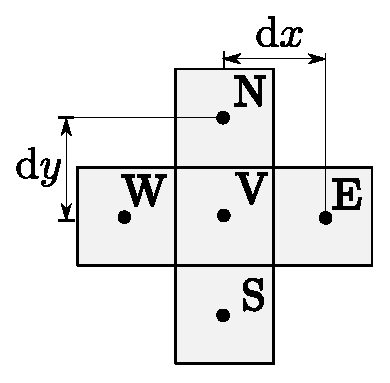
\includegraphics[width=5cm]{fig/nsew.eps}
    \caption{Orientaciones en 2D}
    \label{fig:nsew}
\end{figure}



Se necesita obtener la matriz \texttt{vecindario} que tiene una fila por cada volumen indicando cada uno de sus vecinos y su posición respecto al volumen en cuestión. Identificaremos los bordes aislados con un $0$, los bordes calientes ($T_H$ aplicada) con un $-1$ y los bordes fríos ($T_C$) con $-2$. Para facilitar el armado de \texttt{vecindario} (y que resulte más visual lo que se está haciendo) se podría armar una matriz del dominio. Para el ejemplo tendría la forma:
\begin{equation*}
    \texttt{dominio} = \begin{bmatrix}
    0 &-1 &-1 &-1 & 0 \\
    0 & 1 & 3 & 5 & 0 \\
    0 & 2 & 4 & 6 & 0 \\
    0 & -2 & -2 &-2 &0
    \end{bmatrix}
\end{equation*}
los ceros de las esquinas no tienen ningún significado físico.



Si se elige el orden $[\text{N,W,E,S}]$, entonces para el caso de la figura \texttt{vecindario} tiene la forma 
\begin{equation}
    \texttt{vecindario} =  \begin{bmatrix}
        -1 & 0 & 3 & 2 \\
        1 & 0 & 4 & -2 \\
        -1 & 1 & 5  &4   \\
        3 & 2 & 6 &-2  \\
        -1 & 3 & 0 & 6 \\
        5  & 4  & 0 & -2
    \end{bmatrix}_{\Nvol\times\Ndir}
\end{equation}
osea que los \texttt{vecinos} del volumen 2 son $[1\ms 0\ms 4\ms-2]$. $\Nvol$ es la cantidad de volúmenes y $\Ndir$ es la direccionalidad del problema, en este caso tenemos 4 direcciones porque es un problema plano. Para problemas 3D se tienen 6 direcciones incluyendo las direcciones arriba y abajo [U,N,W,E,S,D].
\clearpage
\begin{lstlisting}[caption = {Armado de la matriz \texttt{vecindario} a partir de la matriz \texttt{dominio}}]
Nvol = max(max(dominio)); % Cantidad de volumenes
[Ny, Nx] = size(dominio(2:end-1,2:end-1));
vecindario = zeros(Nvol,4);
for i=2:Ny+1
	y = (i-2)*dy;  % Se pueden calcular las coordenadas
	for j=2:Nx+1
		x = (j-2)*dx;  % coordenada x
		v = dominio(i,j); 
		if v<1
			continue
		end
		vecindario(v,1) = dominio(i-1,j);
		vecindario(v,2) = dominio(i+1,j);
		vecindario(v,3) = dominio(i,j+1);
		vecindario(v,4) = dominio(i,j-1);
	end
end
\end{lstlisting}

\subsection{Formulación para el método de volúmenes finitos}
Una vez que conocemos el vecindario de los volúmenes se necesita saber que esquema se va aplicar. En este texto se va tratar el esquema implícito o \textit{Euler Backward}.

El problema a resolver es obtener la temperatura del próximo paso de tiempo $T^{m+1}$ usando la temperatura conocida en el paso de tiempo corriente $T^{m}$. Comenzamos despejando para $T^m$ en \eqref{eq:discretizadaImplicita} sin calor generado y teniendo en cuenta que $\Delta x = \Delta y$

\begin{equation} \label{eq:volfin1}
    T_\vol^m =T_\vol^{m+1} - \overbrace{\frac{k S \Delta t}{V \rho \cp\,\Delta x} }^{=\Fourier_x}\left.\sum_i^{\text{caras}}(T_i-T_\vol)\right|^{m+1}
\end{equation}

Nos ha ayudado bastante que sean cuadrados los volúmenes, podemos calcular el número de Fourier por igual para todos los volúmenes. En el caso que no se tengan volúmenes cuadrados se tendrá un número de Fourier en $x$ y otro diferente en $y$
\begin{equation*}
    \Fourier_x= \frac{k S \Delta t}{V \rho \cp \Delta x} = \frac{k \Delta z \Delta y \Delta t}{(\Delta z \Delta x \Delta y) \rho \cp \Delta x} = \frac{k \Delta t}{ \Delta x^2 \rho \cp}
\end{equation*}
de ahora en adelante se usa un único número de Fourier.

Expandiendo \eqref{eq:volfin1}
\begin{equation}
    T_\vol^m =T_\vol^{m+1} + \Fourier(T_\vol^{m+1}-T_\north^{m+1})+\Fourier(T_\vol^{m+1}-T_\west^{m+1})+\Fourier(T_\vol^{m+1}-T_\east^{m+1})+\Fourier(T_\vol^{m+1}-T_\south^{m+1})
\end{equation}
juntando términos nos queda
\begin{equation} \label{eq:volumenesfinitosSolido}
    T_\vol^m = T_\vol^{m+1}(1+4\Fourier) - \Fourier T_\north^{m+1} - \Fourier T_\west^{m+1} - \Fourier T_\east^{m+1} - \Fourier T_\south^{m+1}
\end{equation}

Todas las temperaturas del futuro son incógnitas y por ende se necesita plantear un sistema de ecuaciones y resolver simultáneamente para la temperatura $T^{m+1}$ para todos los volúmenes. La ecuación en forma matricial:

\[
\Cme{T}^{m} =  \Mme{C} \Cme{T}^{m+1}
\]
como lo que nos interesa es $\Cme{T}^{m+1}$, multiplicamos ambos lados por la inversa de la matriz $\Mme{C}$
\begin{equation}
\Cme{T}^{m+1} = \Mme{C} \mldivide \Cme{T}^{m} 
\end{equation}

\subsection[Armado de la matriz \textbf{C}]{Armado de la matriz $\Mme{C}$}

Se arma la ecuación \ref{eq:volumenesfinitosSolido} para cada volumen \textbf{V}, que será una fila en $\Mme{C}$. Hecho en Matlab:
\begin{lstlisting}[caption = {Se arma la matriz $\Mme{C}$ para volúmenes cuadrados.}]
    C = zeros(Nvol);
    Fovec = [Fo Fo Fo Fo];
    for v = 1:Nvol
        vecinos = vecindario(v,:);
        conducen = vecinos ~= 0;
        C(v,v) = 1 + sum(Fovec(conducen));
        C(v,vecinos) = - Fovec(conducen);
    end
\end{lstlisting}
el código de arriba arma la matriz tomando en cuenta los bordes aislados que no conducen. \textbf{Solo usar para una malla donde $\di x=\di y$}. Si se quiere agregar temperaturas fijas o convección hace falta una formulación no especificada aún. Para el caso dado la matriz $\Mme{C}$ no cambia en el tiempo. Con los temas vistos hasta este punto el usuario podría resolver un sistema con condiciones de entorno conocidas y ver como evoluciona en el tiempo. Un ejemplo podría ser fijar la temperatura de un volumen más alto que la de los volúmenes alrededor y dejar al sistema evolucionar hasta la termalización.

\subsection[Vector de flujo de calor]{Vector de flujo de calor \(\Cme{D}\)}
A continuación se tiene el caso del trabajo practico: una placa aislada en sus bordes (N,W,S,E), con calor generado en su parte inferior (Down) y convección en su parte superior (Up). 

Lo que hay que agregar a D son todos los términos de la ecuación de conservación que no dependen de un $T_i$. En este caso la ecuación para cada uno de los elementos es:

\begin{align*} \label{eq:volumenesFinitos3Dejemplo}
    V \rho \cp \frac{(T_\vol^{m+1} - T_\vol^m )}{\Delta t} =\frac{kS}{\Delta x}(T_\west^{m+1} - T_\vol^{m+1}) + &\frac{kS}{\Delta y} (T_\north^{m+1} - T_\vol^{m+1}) +\\ &\QG^{m+1} + \left( \frac{\Delta z}{2 k S} + \frac{1}{\hc S}\right) ( T_{\infty\up} - T_\vol^{m+1})
\end{align*}

La cual luego procesar se vuelve: 

\begin{equation} \label{eq:volumenesfinitosSolidoConZ}
    T_\vol^m = T_\vol^{m+1}(1+4\Fourier+\Fourier_{cz}) - \Fourier T_\north^{m+1} - \Fourier T_\west^{m+1} - \Fourier T_\east^{m+1} - \Fourier T_\south^{m+1} - \QG^{m+1}\cdot\frac{\Delta t}{V \rho \cp} - \Fourier_{cz} T_{\infty\up}
\end{equation}

Donde 

\[Fo_{cz} = \left( \frac{\Delta z}{2 k S} + \frac{1}{\hc S}\right)\cdot \frac{\Delta t}{V \rho \cp}\]

Para lidiar con el calor generado y la convección hay que agregar a la ecuación el vector de flujo de calor $\Cme{D}$ tal que:
\begin{equation}\label{eq:solver}
\Cme{T}^{m+1} =    \Mme{C} \mldivide (\Cme{T}^{m} + \Cme{D}^{m+1})
\end{equation}

Los últimos dos términos de la ecuación \ref{eq:volumenesfinitosSolido} son los que van a parar a $\Cme{D}$ evaluados en el futuro.




\end{document}
